
%%% Local Variables:
%%% mode: latex
%%% TeX-master: theproc
%%% End:

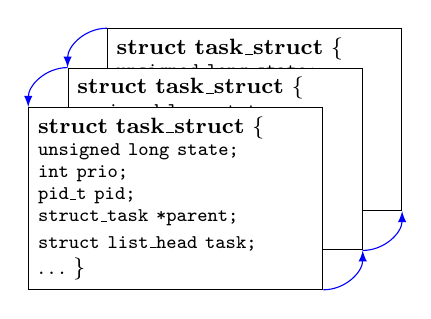
\begin{tikzpicture}
[
pointerpath/.style={blue,->,>=latex,draw},
every node/.style={fill=white,font=\footnotesize,text
  width=3.5cm,draw}
]

\def\structtext{
{\bf struct task\_struct} \{\\
{\scriptsize\tt  
  unsigned long state;\\
  int prio;\\
  pid\_t pid;\\
  struct\_task *parent;\\
  struct list\_head task;}\\
  $\ldots$
\}}  

\foreach \i in {2,1,0} {
  \node (pcb\i) at (.5*\i,.5*\i) {\structtext};
}
\draw[pointerpath] (pcb1.south east) to [bend right=45] (pcb2.south east);
\draw[pointerpath] (pcb0.south east) to [bend right=45] (pcb1.south east);

\draw[pointerpath] (pcb2.north west) to [bend right=45] (pcb1.north west);
\draw[pointerpath] (pcb1.north west) to [bend right=45] (pcb0.north west);

\end{tikzpicture}